\documentclass[twocolumn,12pt]{article}
\usepackage{graphicx}
\usepackage[none]{hyphenat}
\usepackage{hyperref}
\setlength{\columnsep}{8mm}
\setlength{\oddsidemargin}{-1mm}
\setlength{\topmargin}{-20mm}
\setlength{\textheight}{225mm}
\setlength{\parindent}{2mm}
\begin{document}
\title{\bf PROGRESSIVE IMAGE TRANSMISSION}
\author{Akash Kulkarni\\4JC11CS006\and Anurag Kakati\\4JC11CS015\and Ritu S\\4JC11CS090}
\date{\today}
\maketitle
\begin{abstract}
\vspace{-11mm}
\emph{Progressive image transmission is a technique which allows an approximate image to be built up quickly and the details to be transmitted progressively through several passes of the original image. This technique is very useful for picture communication over slow channels. This project implements the PIT technique for colour images of several types.}

\emph{A digital image usually requires great bandwidth or storage for transmission. In order to reduce the bandwidth required for transmitting a given image in a given time, image compression techniques are commonly used to encode images. But even after doing so, lossless compression on average gives us about a two-to-one compression rate.  A better alternative is to send an approximation of each image first, which does not require too many bits but still is sufficiently accurate to give users an idea of what the image looks like. If users find the image to be of interest, they can request a further refinement of the approximation, or the complete image. This is the basic approach behind the progressive image transmission technique that has been implemented in this project.}

\end{abstract}
\section{Introduction}
Progressive Image Transmission is a major application of the multi-resolution approach wherein multi-resolution models generate representations of an image with varying spatial resolution. This usually results in a pyramid like representation of the image, with each layer of the pyramid serving as a prediction model for the layer immediately below.

A simple progressive transmission scheme is to divide the image into blocks and then send a representative pixel for the block. The receiver replaces each pixel in the block with the representative value. Depending on the size of the block, the amount of data that would need to be transmitted could be substantially reduced.
Selecting the representative value for each block can be done in several ways. Two of the methods chosen in this project are:

\begin{itemize}
\item Selecting the top-left pixel of every block.
\item Taking the average of all pixels present in each block.
\end{itemize}

In this project, there are two participants in the transmission: the sender and the receiver. At the sender end, one or more images which may be of varied types and resolutions are selected from the base folder and sent out to the receiver. These images are subjected to compression; which is lossless in this case. As and when the receiver wishes to receive these images, each image is sent to his end in varied levels of clarity which are just about sufficient for him to make out what the image is about. If the receiver finds a level of clarity sufficient, he can command that the transmission of that particular image be stopped then and there and can also select that particular version of image for further need. If the transmission is not interrupted, then after a few more phases, the original image gets received at the receiver end without any loss of the image data. 

\section{Compression}
Images to be sent to the receiver end are first subjected to compression at the sender end. Both compression algorithms implemented are applicable only for images having their heights and widths as integral powers of two. Thus in case of images not satisfying the above criteria, a method called padding is done.

Padding is used to add as many pixels as needed to an existing rectangular image so as to make it have a resolution of height and width both being integral powers of two. The pixels added to expand the image size are given values (0, 0, 0) along the RGB bands which results in black pixel padding. It can further be modified to make it an adaptive method.

Once an image of required resolution is obtained, compression begins. Suppose an image of resolution 64 x 64 is to be compressed. It is first converted to a matrix of order 64 x 64 having a value each for the three bands RGB. These values are then divided into 32 blocks of 2 x 2 and one representative value for each block is obtained using any of the two methods mentioned earlier. It results in another matrix of size 32 x 32. This process continues resulting in many more matrices until finally a matrix of 1 x 1 resolution is obtained.
	
The compression process can be represented as a pyramidal structure. For the given example it can be shown as follows:
\begin{figure}[ht!]
\centering
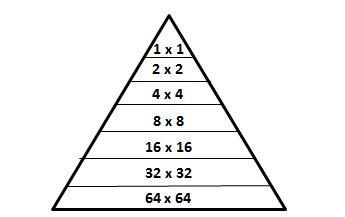
\includegraphics[width=80mm]{tri.jpg}
\end{figure}\\

Thus it can be inferred that for any image scaled to a resolution n x n ;where n is an integral power of 2, after padding, the number of levels of compression can be given by the following formula:

\begin{displaymath}
L = log_2 \hspace{2pt} n
\end{displaymath}

\section{Transmission}
Once the image has been compressed to L levels, as and when the receiver requests for the image, transmission phase begins. It starts with sending of the image having the highest level of compression. The remaining compressed versions of the image are sent further on, that too only if the receiver requires it.

There are three cases in which the transmission phase can end:
\begin{itemize}
\item At any point of time, if the user realizes that the image is not of his interest, he can terminate the transmission of that particular image and move onto the next one.
\item If the user finds that an intermediate version of the image is sufficient for his use, he can abort the transmission and select that image.
\item The user can wait to receive the complete original image without any compression.
\end{itemize}
%\hspace{15mm}
\section{Decompression}

Once the sender transmits a compressed version of the image, it needs to be decompressed at the receiver end. The main characteristic of a decompressed image is that it is of the same size as that of the original image. This is achieved by proportionately scaling up the received smaller-sized matrices to the original width and height by repeating pixels in each block with the corresponding values in the smaller matrix. 
	
This matrix conversion is done for all 3 bands of colours and finally the colour band matrices are subjected to a function to convert it back to the image format that is ultimately displayed to the user. 

\section{Performance Evaluation}

As this is a just a simulation of the actual transmission of an image over a network, transmission speed cannot be taken into account for performance evaluation. But it is possible to track the progression of an image that is transmitted by plotting a graph of the various compression levels vs. the intermediate sizes.

For a sample image(symbol.jpg: 64 x 64, 1.5kB), the progression is plotted as follows:\\\\\\

\begin{figure}[ht!]
\centering
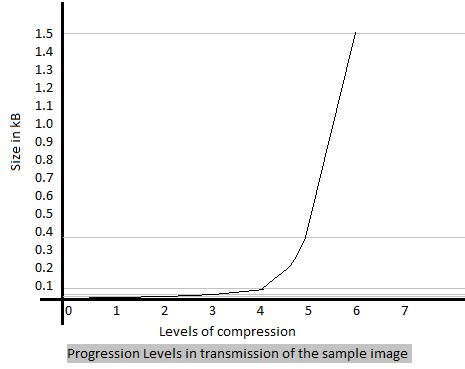
\includegraphics[width=80mm]{g1.jpg}
\end{figure}

As seen from the graph, the size of the intermediate images at each level is exponential increasing. This gives an idea about how much storage space can be saved if the user is satisfied with an image even a single level prior to the final level.

Also, the following table gives statistics regarding the accuracy of both the algorithms. It can be verified that at the final level, lossless compression has indeed been achieved.\\


\begin{tabular}{|c|c|c|}
\hline
Image Name&BC&After DC\\
\hline
tiger.jpg&384.0kB&384.0kB\\
\hline
galaxy.jpg&91.55kB&96.0kB\\
\hline
Sonic.png&18.5kB&24.0kB\\
\hline
apple.jpg&384.0kB&384.0kB\\
\hline
\end{tabular}\\\\

Incase of padded images the final size increases by a small amount than the original size. It depends on how far off the image initially was from satisfying the criteria. \\\\
\begin{tabular}{|c|c|c|}
\hline
Padded Image&Original Size&Increse in size\\
\hline
ipad.jpg&384.0kB&0.0kB\\
\hline
galaxy.jpg&91.55kB&4.45kB\\
\hline
Sonic.png&18.5kB&5.5kB\\
\hline
Cs.bmp&63.2kB&32.8kB\\
\hline
\end{tabular}\\\\

These algorithms were found to work on .jpeg, .png and .bmp images. It was also observed that there was not much of a perceivable difference of the image clarity for the images generated by the two different algorithms.
\section{Simulated Results}

\begin{figure}[ht!]
\centering

\includegraphics[width=40mm]{tig2.jpg}
\end{figure}\begin{figure}[ht!]
\centering

\includegraphics[width=40mm]{tig3.jpg}
\end{figure}
\begin{figure}[ht!]
\centering
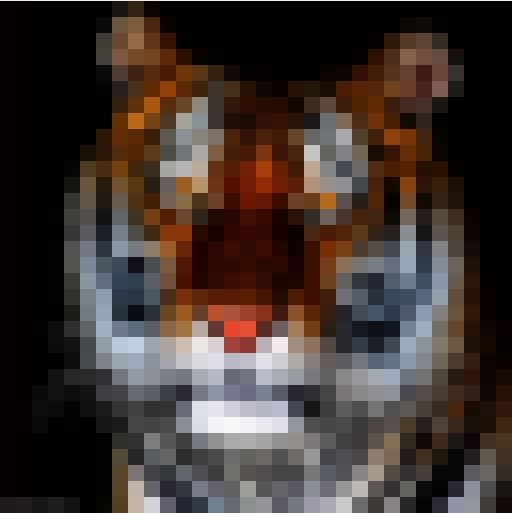
\includegraphics[width=40mm]{tig4.jpg}
\end{figure}
\begin{figure}[ht!]
\centering
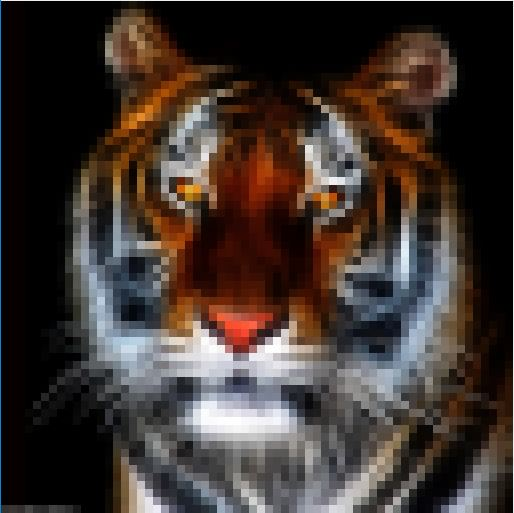
\includegraphics[width=40mm]{tig5.jpg}
\end{figure}
\begin{figure}[ht!]
\centering

\includegraphics[width=40mm]{tig6.jpg}
\end{figure}
\begin{figure}[ht!]
\centering
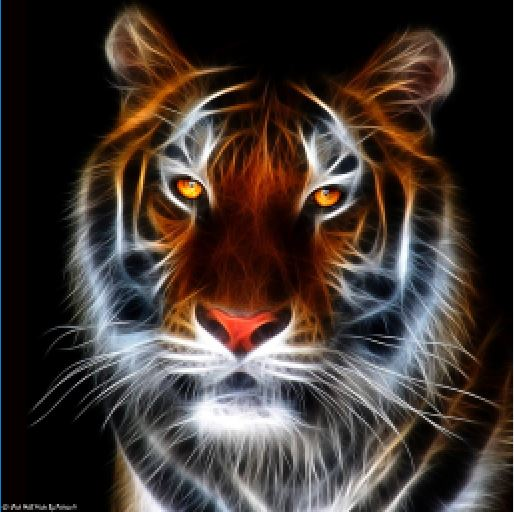
\includegraphics[width=40mm]{tig7.jpg}
\end{figure}
\begin{figure}[ht!]
\centering
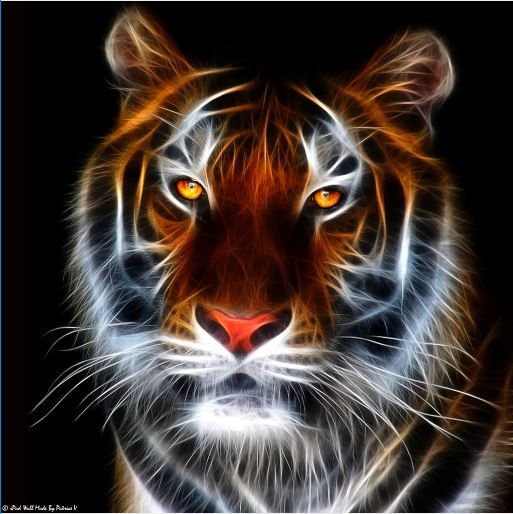
\includegraphics[width=40mm]{tig8.jpg}
\end{figure}

\vspace{30mm}
\begin{thebibliography}{9}
\bibitem{1}www.stackoverflow.com
\bibitem{2}http://docs.oracle.com/javase/7/docs/api/
\bibitem{3}\emph{Head First JAVA} - Kathy Sierra and Bert Bates
\bibitem{4}\emph{Introduction to Data Compression} - Khalid Sayood
\end{thebibliography}
\end{document}